\documentclass[varwidth, border=0pt]{standalone}

\usepackage{times}      % Loads the Times-Roman Fonts
\usepackage{mathptmx}   % Loads the Times-Roman Math Fonts
\usepackage{subcaption}
\usepackage[labelfont={bf,sf},%
labelsep=period,%
justification=centering,
labelformat=parens,labelsep=quad,skip=3pt,font=scriptsize]{caption}
\usepackage{graphicx}

\begin{document}
	
	\begin{figure}
	\centering
    \begin{subfigure}{0.5\textwidth}
        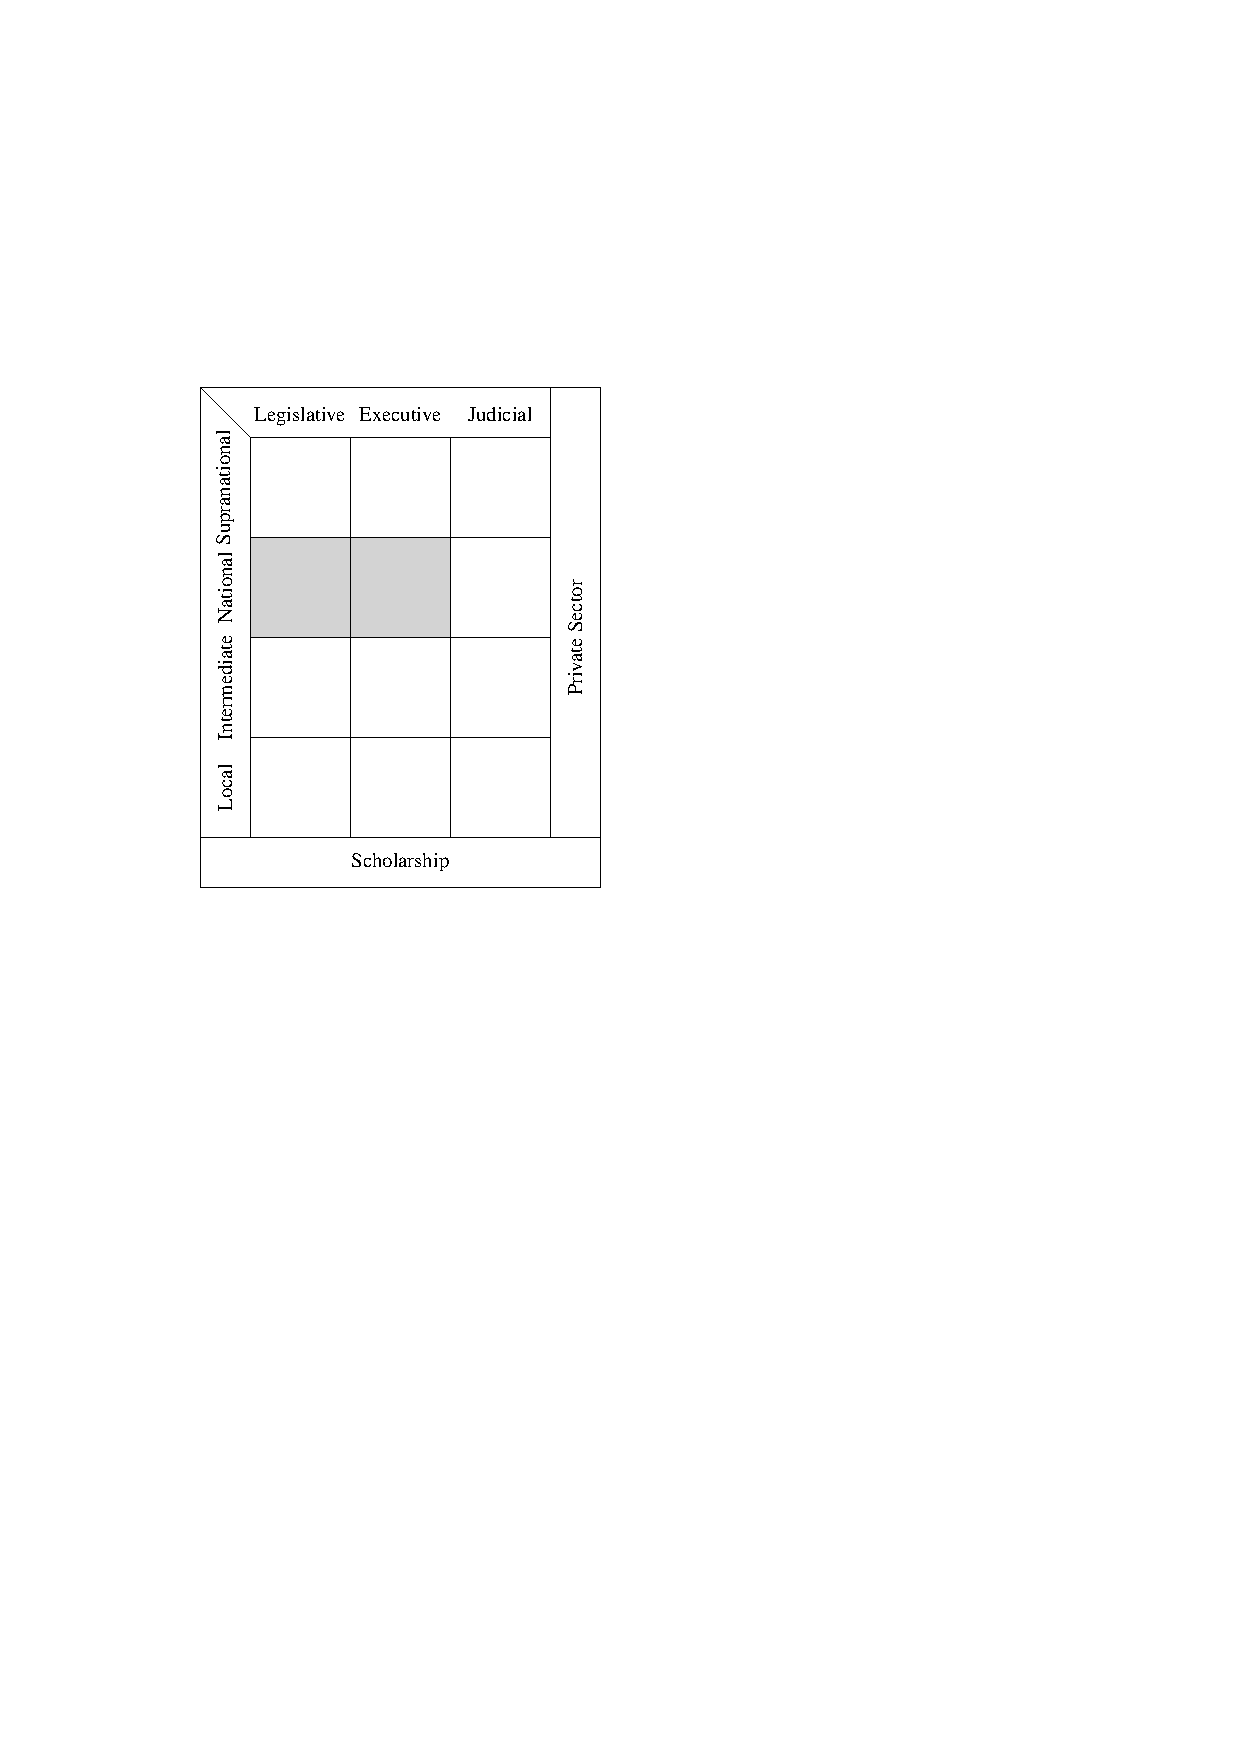
\includegraphics[width=\textwidth]{../../graphics/legal-system-structure.pdf}
        \subcaption{Overview of the legal system}
    \end{subfigure}%
    \begin{subfigure}{0.5\textwidth}
        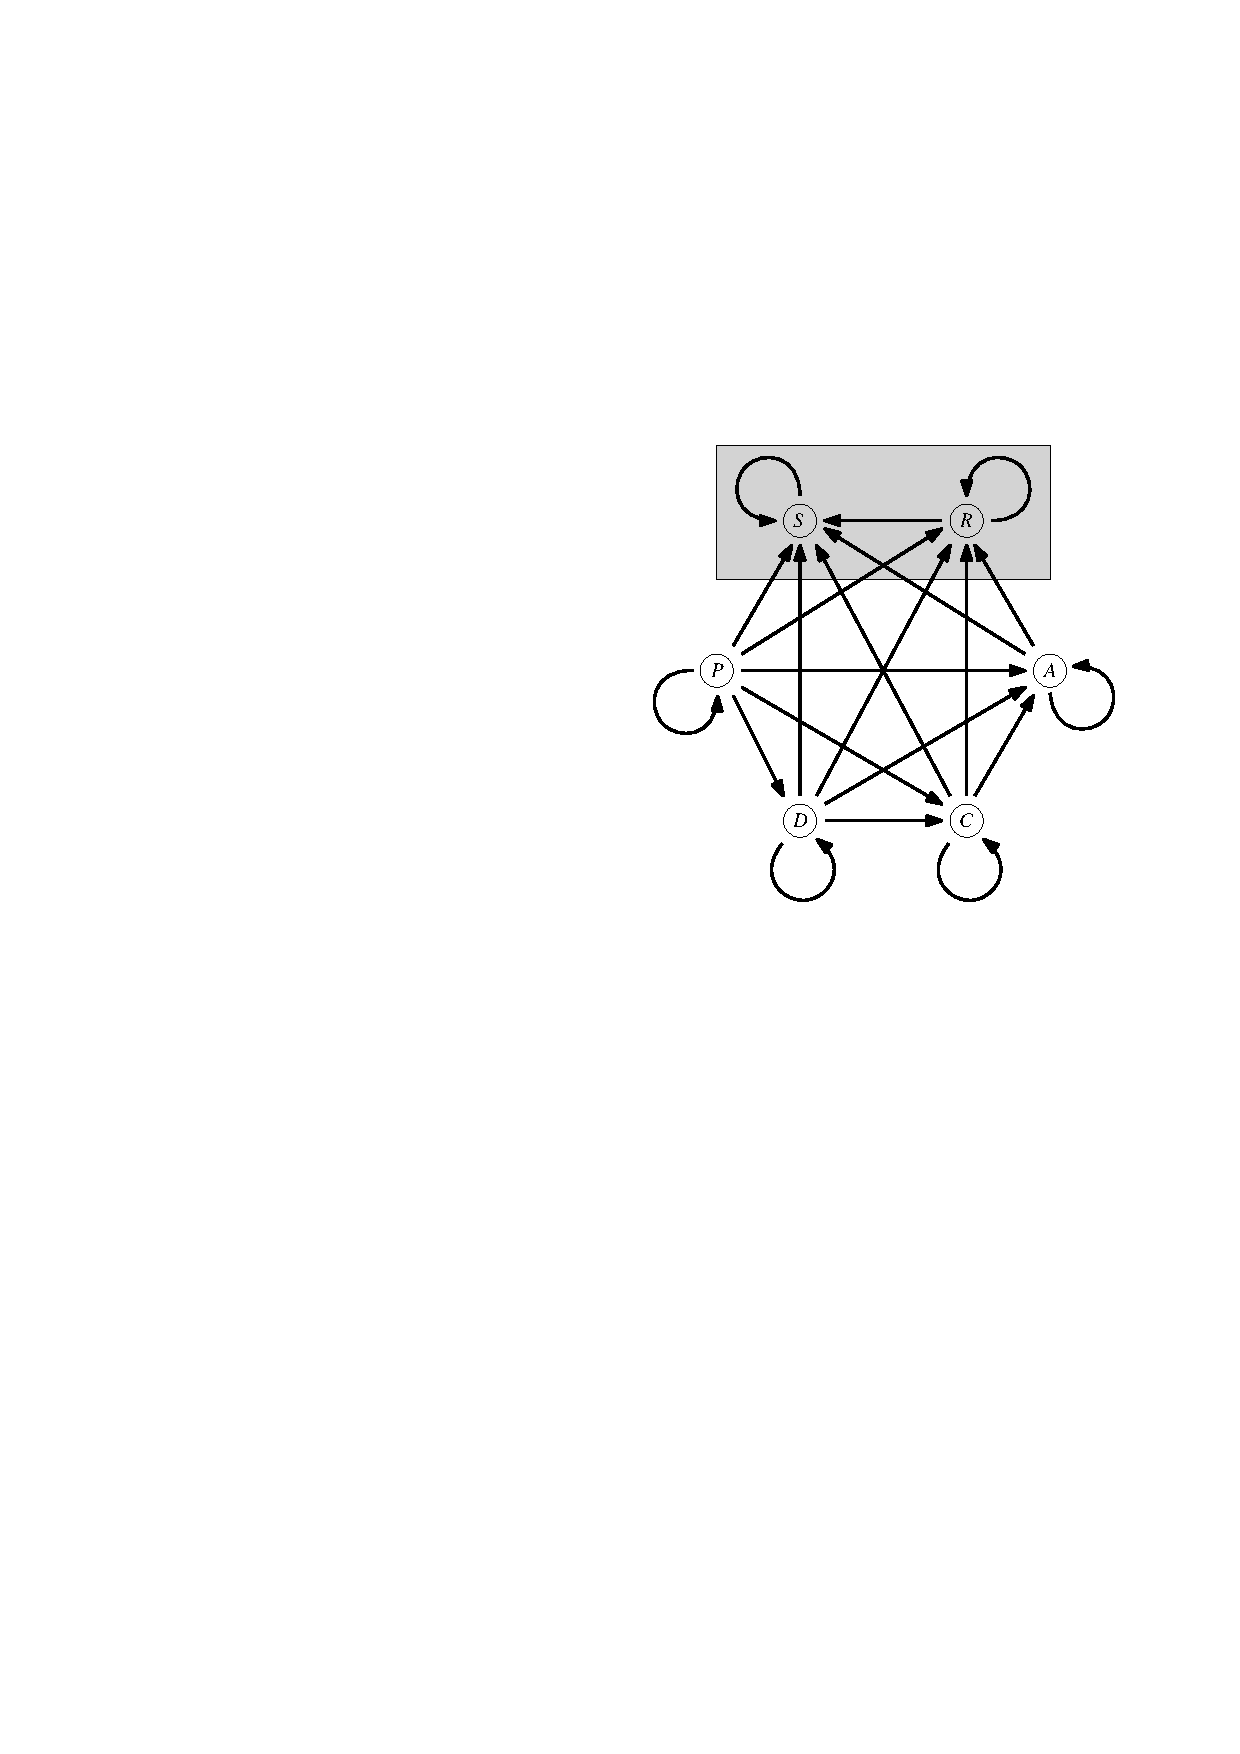
\includegraphics[width=\textwidth]{../../graphics/legal-system-relationships.pdf}
        \subcaption{Potential dependencies between typical legal outputs}
    \end{subfigure}
    \end{figure}
	
\end{document}